

\setcounter{section}{1}
\section{Project Overview}
\bigskip
\subsection{System Overview}
\medskip
The Akriveia Beacon indoor locating rescue system combines hardware, electrical, and software systems to detect and locate multiple occupants within a building during an emergency disaster situation. Each individual component of the system is developed separately in the Proof of Concept (PoC) phase, partially integrated in the Prototype phase and fully integrated in the Final Product phase. 

\bigskip
A high-level system overview presents three Locator Beacons, an ID tag, a data processing unit, and a graphical user interface (Figure \ref{sys_arch}). Using the Time-of-Flight principle (\Gls{ToF}) which is a method for measuring distances between transceivers. Based on the time difference between the emission of a signal after being reflected by an object and its return to the sensor, the distance between a beacon and an ID tag can be estimated r\cite{R2-0}. 

\bigskip
The Locator Beacons transmit ultra-wideband (UWB) signals in the frequency of 3.5-6.5GHz to the ID tag to acquire a response. When the response returns back to the Beacon a ToF measurement is acquired. The ToF data captured by ESP32 microcontroller unit(\Gls{MCU}) will be forwarded to a portable data processing unit, a Raspberry Pi, via private WiFi network with User Datagram Protocol (\Gls{UDP}). Then the processing unit will calculate the distance and coordinates of the ID tags using a trilateration algorithm, then the coordinates results are displayed on a Graphical User Interface (\Gls{GUI}) for operators.


\medskip
\begin{figure}[H]
\centering
    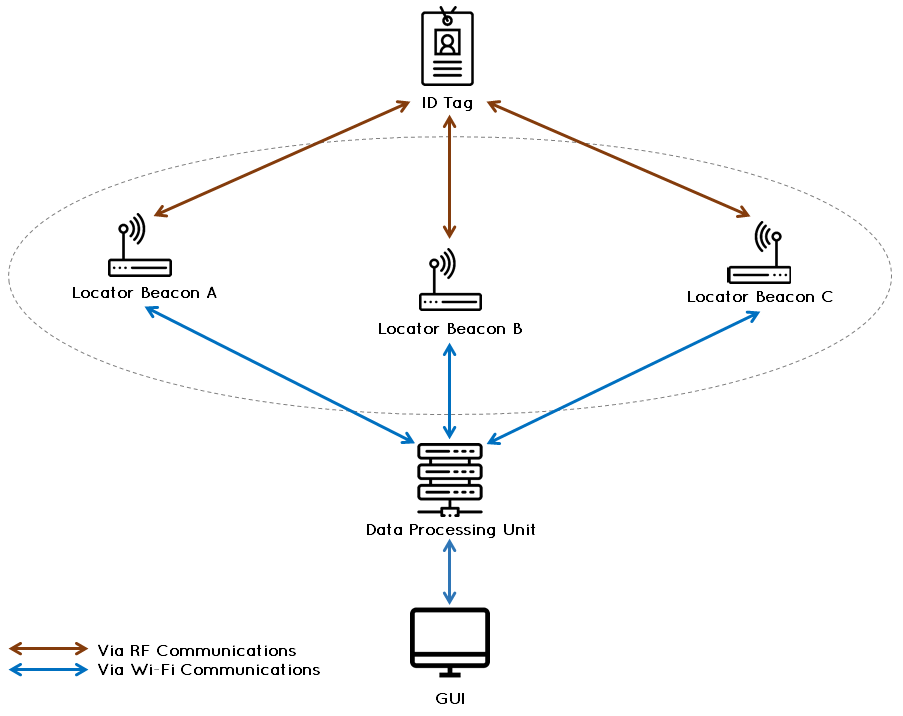
\includegraphics[scale=0.60]{./images/00_sys_arch.png}
    \caption{High Level System Layout}
    \label{sys_arch}
\end{figure}
\pagebreak

The final product will demonstrate the fully functional indoor rescue system that detects the location of the ID tags and displays it accordingly on a GUI. Here the of ESP32’s WiFi modules for Beacon to DPU communications can be seen (Figure \ref{final}), as the Beacon will communicate via WiFi communication with the data processing unit. The WiFi network will be a closed private network meaning that the network is only share between beacons and the data processing unit to ensure security, reliability and stability. Furthermore, implementation of a RF harvesting circuit for charging the ID Tag device during deep sleep mode will occur throughout this stage. All the components of the systems will be fully integrated as a close-to-production product. Component circuits and \Gls{PCB} footprint will be minimized and proper casing will be made to house all electronics. The data processing unit will provide the user with a full GUI to interact with along with fully implemented features such as importable blueprints and system configurations.

\bigskip
\begin{figure}[H]
\centering
    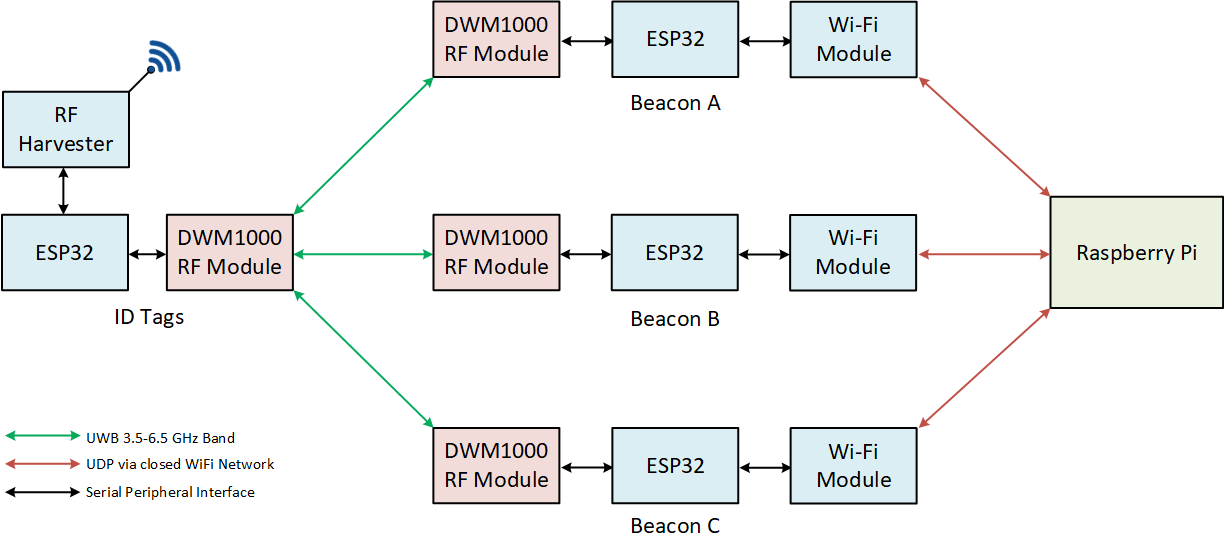
\includegraphics[width=\linewidth]{./images/03_final.png}
    \caption{Final System Block Diagram}
    \label{final}
\end{figure}

\pagebreak
\subsubsection{System Components}
\medskip
The Beacon and ID tags are composed of Decawave DWM1000 \Gls{UWB} module (Figure \ref{dwm_esp} right) and a Espressif ESP32 microcontroller (Figure \ref{dwm_esp} left). The ESP32 contains a Tensilica Xtensa LX6 microprocessor in both dual-core and single-core variations and includes a in-built antenna, power amplifier, low-noise receive amplifier, filters, and power-management modules. The DWM1000 is an IEEE802.15.4-2011 UWB compliant and \Gls{FCC}/\Gls{ETSI} certified wireless transceiver module based on Decawave’s DW1000 IC \cite{R2-1-1-1}. This module is a combination of DW1000 \Gls{IC}, a built in antenna, power management system, and clock control for simple design integrations. 

\medskip
\begin{figure}[H]
\centering
    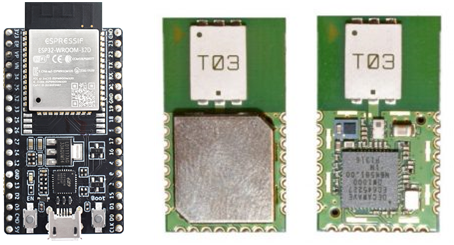
\includegraphics[scale=0.75]{./images/dwm_esp.png}
    \caption{Left ESP32 \cite{R2-1-1-2}, Right DWM1000}
    \label{dwm_esp}
\end{figure}

The Data Processing Unit is a stand alone single board computer (\Gls{SBC}). For the demonstration of this project a Raspberry Pi 3 B+ is used as the data processing unit (\Gls{DPU}) since it is an affordable and robust SBC, but the DPU in theory could be any electrical computer device that is capable of running a basic linux operating system; as the software stack for the DPU is designed to operate on any linux based system. The Raspberry Pi 3 B+ is affordable, portable, and designed with an Cortex-A53 processor, it satisfy the minimum requirements for the DPU.

\medskip
\begin{figure}[H]
\centering
    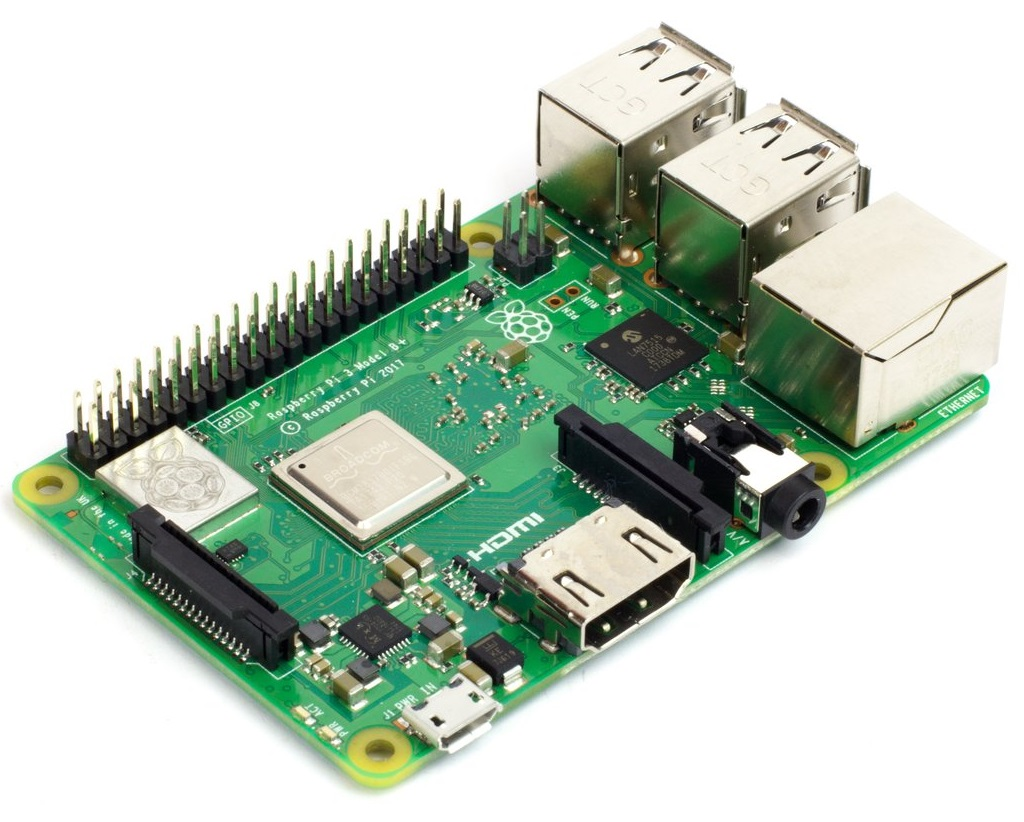
\includegraphics[scale=1]{./images/pi.jpg}
    \caption{Raspberry Pi 3 B+ Model \cite{R2-1-1-3}}
    \label{pi}
\end{figure}



\pagebreak
\subsubsection{Trilateration Method}
\medskip
The Akriveia Beacon 2-D indoor localization solution determines the X-Y coordinates of ID tags using basic trilateration methods. The trilateration method follows a lateration scheme with absolute distances, which uses distance related metrics such as ToF to determine the distance between a sender and a receiver. In the case where there is a single beacon and ID tag, the distance between the two entities can be interpreted as the radius of a circle traced with the beacon centered as demonstrated in figure \ref{tri} with D is the distance between any given ID Tag and Beacon. 

\medskip
\begin{figure}[H]
\centering
    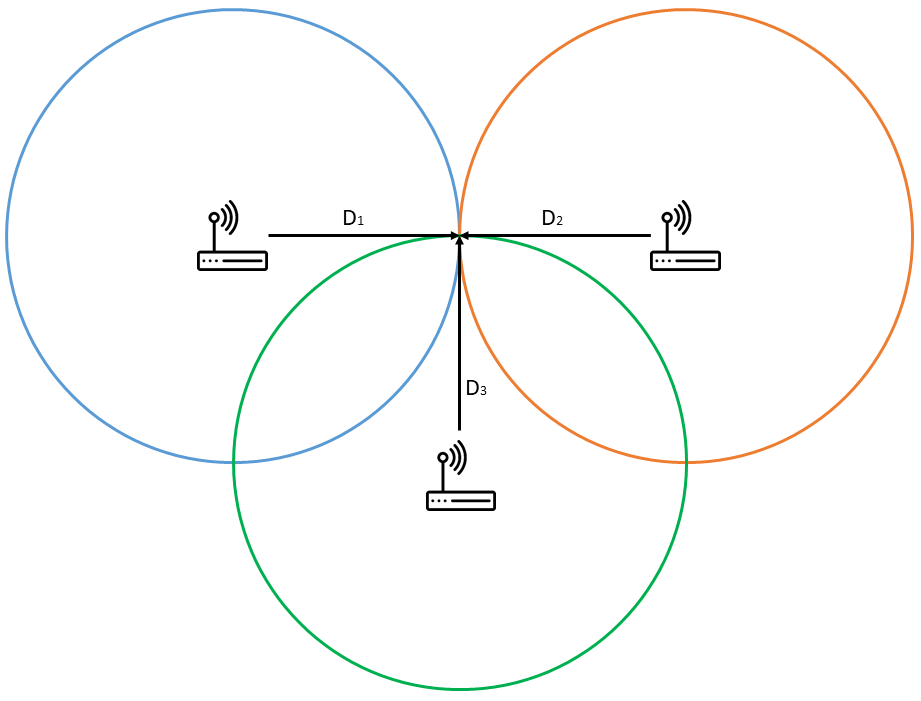
\includegraphics[scale=0.55]{./images/Tri.png}
    \caption{Trilateration Diagram}
    \label{tri}
\end{figure}


\medskip
Such a circle takes on a standard mathematical form as shown in equation (1) below \cite{R2-1-2-1}, where variables $x_0$ and $y_0$ are the 2-D coordinates of the beacon position relative to its environment, and $r_0$ is the distance between the beacon and the ID tag. Given the 2-D coordinates the three beacons and their individual distance with respect to the ID tag, three circles can be traced to form an intersection point at the location of the ID tag. Hence, three standard form circle equations are generated to form a system of equations with two unknowns as shown in equation (2). The solution to the unknowns, or the intersection coordinates of the ID tag can be obtained by solving the system in equation (2).


\medskip
\begin{equation}
	(x-x_{1})^2 + (y-y_{1})^2 = r_{0}^2
\end{equation}

\begin{gather}
	(x-x_1)^2 + (y-y_1)^2 = {r_1}^2 \\
	\nonumber (x-x_2)^2 + (y-y_2)^2 = {r_2}^2 \\
	\nonumber (x-x_3)^2 + (y-y_3)^2 = {r_3}^2  
\end{gather}


\pagebreak
\subsection{Project Scope}

\medskip
\textbf{Goal}

\medskip
The goal of the Akriveia Beacon system is to provide accurate and reliable indoor location tracking of trapping personnel during small scale emergency disaster in near real time. The location information will be complied and presented to aid first responders on locating trapped victims during any emergency disaster situations. By providing accurate location data of trapped victims, the search and rescue time for first responders can be drastically lowered, and therefore, limit first responder exposure to potentially dangerous environments and increase the chances of survival of trapped victims.

\bigskip
\textbf{Justification}

\medskip
The Akriveia Beacon system must maintain critical functions under emergency disaster situations such as fires and low magnitude earthquakes. System components must design to be durable and initiative to use for all end users. Each beacon and ID tag must be designed to withstand various environmental factors such as high temperature, low visibility, and other dangerous factors. The users of the system must have some form of knowledge of the system prior to operating. Lastly, as an indoor tracking tag device the ID tags must be worn at all times by all personnel associated.

\bigskip
\textbf{Assumptions}

\medskip
The Akriveia Beacon system must maintain critical functions under emergency disaster situations such as fires and low magnitude earthquakes (less than 6.9 on Richter magnitude scale). Each beacon and ID tag must be designed to withstand various environmental factors such as high temperature, low oxygen, fragile structural integrity, and other dangerous factors. The users of the system must have some basic form of technical and operational knowledge of the system prior to operating. Lastly, as an indoor tracking tag device the ID tags must be worn at all times by all personnel associated within the intended area of operations.

\bigskip
\textbf{Deliverables}

\medskip
The Akriveia Beacon is designed as a system of anchor beacons and wearable ID tags composed of Espressif ESP32s MCUs and Decawave DWM1000 UWB transceiver modules. A minimum of three beacons are needed for trilateration to function. A portable data processing unit will also be part of the system and be implemented in Rust to create a layer of control and interaction between the users and the system. For the purpose of the demonstration a Raspberry Pi 3 B+ will be used as the DPU. In theory, any single board computer which meets the minimal specification can be used as the DPU.

\bigskip
\textbf{Constraints}

\medskip
The system as a whole must remain operational throughout the event of a disaster as the search and rescue effort rely on information generated by the system. Each component of the system will need a battery backup to maintain functionality if the primary power source is unavailable. As an indoor location tracking system a tag device must be worn by personnel being tracked at all times while in proximity of the beacons. As wearable electronics, the size of the ID tags must be optimized in its design so it is ergonomical as an everyday carry item. Power consumption will be another important aspect to focus on as with all wearable electronics. To reduce maintenance costs the device battery must maintain charge over prolonged periods of time or have methods of wireless charging. 



\pagebreak
\subsection{Risks}
\medskip
As a system that will operate in potentially dangerous environments during disasters the Akriveia Beacon system faces various boundaries, which can be a source of risk and thus potential risks and boundaries should be defined further. 

\bigskip
Most common risks for this project are:

\begin{itemize}
\setlength\itemsep{0.1mm}
	\item \textbf{Cost Risk:} Typically escalation of project costs due to poor cost estimating accuracy and scope creep.
	\item \textbf{Schedule Risk:} The risk that activities will take longer than expected. Slippages in schedule typically increase costs and delay the receipt of project benefits, with possible loss of competitive advantage.
	\item \textbf{Performance Risk:} The risk that the project will fail to produce results consistent with project specifications.
	\item \textbf{Governance Risk:} Relates to board and management performance with regard to ethics, community stewardship, and company reputation.
	\item \textbf{Strategic Risks:} From errors in strategy, such as choosing a technology that cannot be made to work.
	\item \textbf{Operational Risk:} includes risks from poor implementation and process problems such as procurement, production, and distribution.
	\item \textbf{Market Risks:} include competition, foreign exchange, commodity markets, and interest rate risk, as well as liquidity and credit risks.
	\item \textbf{Legal Risks:} arise from legal and regulatory obligations, including contract risks and litigation brought against the organization.
	\item \textbf{External Hazards Risks:} Including fire, storms, floods, earthquakes; vandalism, and sabotage.
\end{itemize}

Some important physical and operational risks with the Akriveia Beacon system highlighted are, the resolution accuracy of the indoor location system, failure to carry ID tag during disasters, system integrity during hazardous environments. These risks are associated with system operation and mitigation strategies are developed to reduce the occurrence and impact of these types of risks. Risks relating to the overall project are considered and analyzed in the tables below. The team at TRIWAVE SYSTEMS will perform in depth analysis of all possible risk of the project and create mitigation strategies to best minimize these risks of the project.

\medskip
\begin{table}[H]
\centering
\def\arraystretch{1.2}
\begin{tabular}{ | m{1.5cm} | m{4cm}| m{2cm} | m{7.5cm}|}
\hline
\rowcolor{lightgray} \textbf{Severity} & \textbf{Risk} & \textbf{Likelihood} & \textbf{Mitigation Strategy}\\
\hline
Low & Feature creeping inflates the scope of the project. & Medium & Team members all agree on the scope of the product and new features will be further analysed on feasibility and cost/benefit ratio before adding to project.\\
\hline 
Low & Team members misinterpret projects requirements. & Low & Requirement documents details concise and clear requirements of the project to minimize misinterpretation during development.\\
\hline
Low & Insufficient project funding & Medium & A self-funded budget has been established and if needed each member can provide additional funding for the project.\\
\hline
\end{tabular}
\caption{Project Risk Assessment Table - Part 1}
\end{table}	

\pagebreak
\begin{table}[H]
\centering
\def\arraystretch{1.3}
\begin{tabular}{ | m{1.6cm} | m{4cm}| m{2cm} | m{7.4cm}|}
\hline
\rowcolor{lightgray} \textbf{Severity} & \textbf{Risk} & \textbf{Likelihood} & \textbf{Mitigation Strategy}\\
\hline
Moderate & Targeted end users have difficulties interacting the system user interface. & Medium & The project will include two phases of usability testing to ensure UI interaction is intuitive. The first with team members as the evaluators and the second with external evaluators. \\
\hline
Moderate & Team member unavailable to perform duties due to illness or unforeseen circumstances. & Medium & Team members are familiar with the core architecture of the system, and with difference domain of expertise all member can be covered by each other, in case of illness or unforeseen circumstances. \\
\hline
Moderate & Miscalculate Project time line, failure to meet project deadlines & Low & Proper project planning strategies such as grant charts and project management techniques will mitigate delays and other unforeseen circumstances. \\
\hline
Moderate & Target audience may not find final product as initiative or easy to use. & Low & Constant communication and feedback between team members and stakeholders can mitigate this risk. \\
\hline
Moderate & System cost may be too expensive for consumers to consider to purchase. & High & As this technology is still in its infancy cost is a major concern, in the future with more refined technology can lower cost along with government incentive for more potential consumers. \\
\hline
Significant & Delay of project due to delay in component purchasing, manufacturing, and shipping. & Medium & Plan purchase dates as early as possible, research multiple vendors and backup component sources. \\
\hline
Significant & Stakeholders incoherent with project definition and scope. & Low & The team will provide clear and coherent communication and project description with shareholders to avoid misinterpreted ideas. \\
\hline
Significant & Targeted location resolution accuracy of 50 cm cannot be achieved. & Low & Create alternative solution to best fit the scope of the project without compromising the integrity of the core system. Such as lowering resolution to 5m zone instead.\\
\hline
Significant & Beacon is destroyed or is offline due to external hazards during emergency disaster after system deployment. & High & The system needs minimal three beacons to operate, in ideals situation there are multiple redundant backup beacons to keep system operational during disasters. \\
\hline
Significant & Location of ID tags generate inaccurate data and increase  search and rescue time & Low & The system will be calibrated for each environment and system test drills can be performed to ensure that the system can produce accurate and reliable data. \\
\hline
\end{tabular}
\caption{Project Risk Assessment Table - Part 2}
\end{table}	


\pagebreak
\subsection{Benefits}
\medskip
The Akriveia Beacon was envisioned as a system to aid first responders in search and rescue operation during small scale disaster situations. As an indoor location tracking system designed for emergency search and rescue operations, the Akriveia Beacon is the first of its kind. The core feature is the near real time tracking of ID tags upto a distance resolution of 50 cm, which is substantial since no system exists with a similar purpose and application. One major benefit of the system is to reduce search and rescue operation time. In dangerous environments during an emergency disaster first responders are exposed to various hazards which creates considerable amount of risk to their lives. To minimize the first responders’ and the trapped victims' exposure to these environments is critical. By providing near real time location of trapped victiums the search time is significantly reduced allowing for quicker rescue procedures to be carried out.

\bigskip
Another advantage of the Akriveia Beacon system for the end users is that it provides a simple and intuitive graphical user interface. A clear and intuitive Graphical User Interface (\Gls{GUI}) allows for the first responders to quickly understand and interpolate location coordinates of trapped victims and relay this important information directly to the first line of fire fighters heading into the targeted building. Clarity minimized potential mistakes and error which is pivotal in search and rescue operations.

\bigskip
The Akriveia Beacon system could also generate substantial economic benefits if it were to become a successful product. Successful sales of this product would generate profit which allows for the growth of TRIWAVE SYSTEMS. As well as the build up a brand and company reputation in the industry to further create a multitude of business opportunities. This growth will allow the Akriveia Beacon system to be further refined and improved upon to become an even more robust and reliable system which would revolutionize emergency search and rescue operations.

\bigskip
The final product version of Akriveia Beacon can be further be improved upon to include a vast range of potentials. One major implementation for the system considered was a central cloud management system. Since each beacon has the capability to access any WiFi network, a central cloud server could utilize this feature to create a management system for each individual building installed with the Akriveia Beacon system. A central management system allows for upwards scalability and improved process for system access and maintenance.




